\chapter{Software cloud-based}\label{ch-05}

\lecturemeta{Capitolo originale: 5 --- Cloud-based Software \quad\textbullet\quad Antonio Brogi}{Appunti di Emiliano Sescu (github.com/Faxatos), cap. 5}

La rivoluzione del software cloud-based nasce dall'unione di due cose:
hardware potente e reti ad alta velocità, che hanno portato al
\textbf{cloud computing}, e \textbf{risorse virtualizzate} (calcolo,
storage, piattaforme) disponibili su richiesta.

I vantaggi principali del software nel cloud sono:

\begin{itemize}
\tightlist
\item
  \textbf{Scalabilità} (\emph{scalability}): mantenere le prestazioni
  quando il carico aumenta (utile quando non si sa quanti clienti avrà
  il prodotto).
\item
  \textbf{Elasticità} (\emph{elasticity}): adattare la configurazione
  dei server alla domanda che cambia, evitando sia di avere
  \textbf{troppe} risorse (\emph{overprovisioning}) sia \textbf{troppo
  poche} (\emph{underprovisioning}).
\item
  \textbf{Resilienza} (\emph{resilience}): continuare a fornire il
  servizio anche se alcuni server si guastano.
\item
  \textbf{Costo}: la maggior parte dei servizi cloud si paga a consumo
  (\emph{pay-per-use}), senza comprare hardware.
\end{itemize}

\section{Virtualizzazione e
container}\label{virtualizzazione-e-container}

Uno degli ingredienti del cloud è la virtualizzazione delle risorse.
Nello stesso server fisico si possono ospitare molti \textbf{server
virtuali}, cioè \textbf{macchine virtuali} (VM).

\begin{figure}[H]
\centering
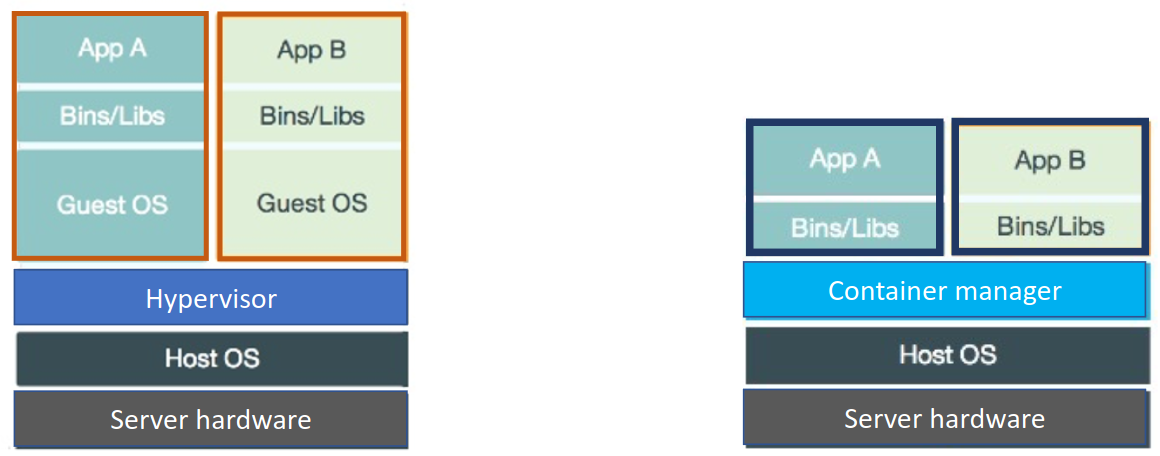
\includegraphics[width=0.80\linewidth,height=0.45\textheight,keepaspectratio]{images/05-cloud_fig5-1_vm-e-container.png}
\caption{Macchine virtuali e container.}
\end{figure}

Lo stack a sinistra in Fig. 5.1 è una macchina con un sistema operativo
e un \textbf{hypervisor}, il software che rende possibile la
virtualizzazione. Quello in figura è un hypervisor di \textbf{tipo 2}
(\emph{hosted}), che gira sopra il sistema operativo; quello di
\textbf{tipo 1} (\emph{bare-metal}) gira direttamente sull'hardware. I
riquadri arancioni sono le macchine virtuali, cioè partizioni della
macchina fisica, ognuna con il proprio sistema operativo (\emph{guest
OS}).

Lo stack a destra usa i \textbf{container}: invece di isolare tutto come
fanno le VM, i container \textbf{condividono lo stesso sistema
operativo} e sfruttano la capacità del kernel di creare più istanze
isolate dello spazio utente. I container girano su un \textbf{container
manager} che sta sopra il sistema operativo.

\begin{boxtip}{VM vs container}

Condividere il sistema operativo rende i container \textbf{molto più
leggeri e veloci da avviare} delle VM. Il prezzo è una \textbf{sicurezza
minore}: c'è meno isolamento, e ad esempio un container può
``contaminare'' la memoria di un altro.

\end{boxtip}

\subsection{Docker}\label{docker}

La \textbf{portabilità} delle applicazioni è sempre stata uno dei grandi
problemi dell'ingegneria del software. Tradizionalmente c'era un
ambiente per sviluppo e test e un altro per la produzione (quello in cui
l'applicazione viene installata e distribuita agli utenti). I due
ambienti non erano uguali, quindi ogni volta che un'applicazione passava
da uno all'altro servivano tempo e soldi.

\begin{boxdefinition}{Docker}

\textbf{Docker} è una piattaforma che permette di eseguire applicazioni
in un ambiente isolato, usando i \textbf{container}. Un'applicazione,
una volta sviluppata, viene chiusa in un container: aperto in un nuovo
ambiente, il container non ha problemi di portabilità grazie al
\textbf{Docker Engine} (che crea ed esegue i container). La piattaforma
include anche il \textbf{Docker Hub}, per distribuire i container.

\end{boxdefinition}

\begin{figure}[H]
\centering
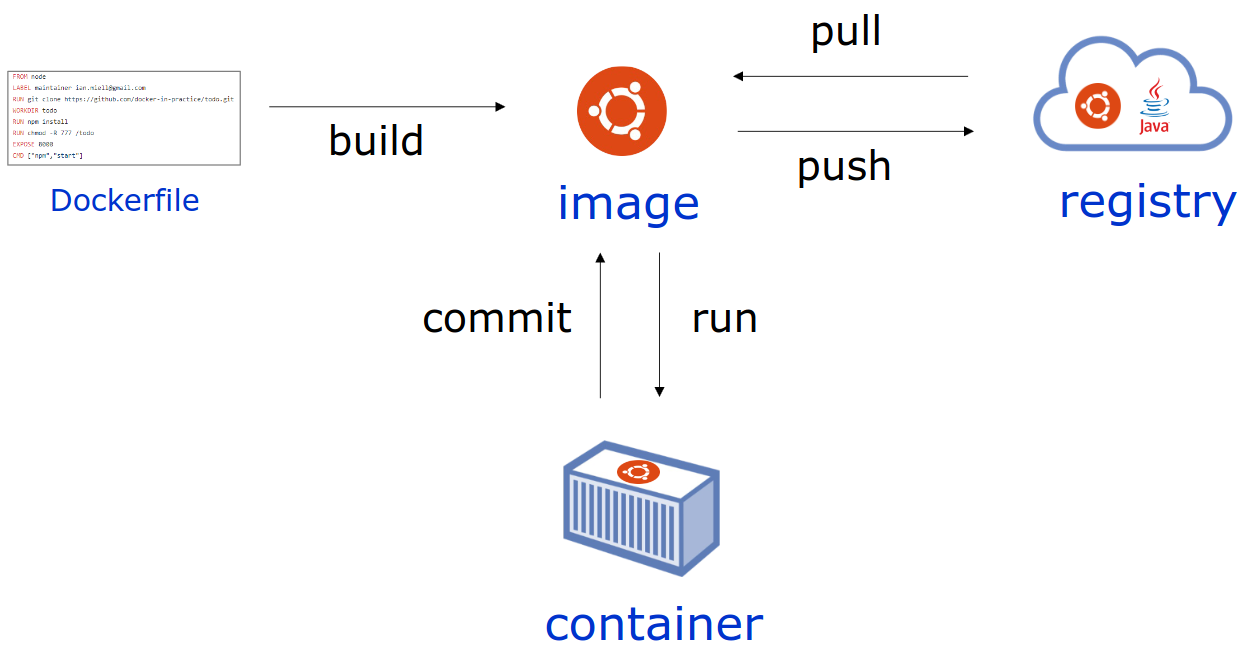
\includegraphics[width=0.80\linewidth,height=0.45\textheight,keepaspectratio]{images/05-cloud_fig5-2_ciclo-docker.png}
\caption{Il ciclo di vita di Docker.}
\end{figure}

I componenti software vengono impacchettati in \textbf{immagini}
(\emph{image}), cioè modelli \textbf{in sola lettura} usati per creare
ed eseguire i container. Siccome le immagini sono in sola lettura, per
salvare dati in modo persistente servono dei \textbf{volumi esterni}.

Le immagini sono conservate in un \textbf{Docker registry} (privato o
pubblico), organizzato in \textbf{repository}: ogni repository contiene
le immagini delle diverse versioni di un software, identificate dalla
coppia \texttt{repository:tag}. Le immagini sono fatte a
\textbf{livelli} (\emph{layer}), e ogni livello è a sua volta
un'immagine (quello più in basso si chiama \textbf{immagine base}).

I comandi principali (Fig. 5.2) sono:

\begin{itemize}
\tightlist
\item
  \texttt{pull}: scarica un'immagine dal registry;
\item
  \texttt{push}: carica un'immagine nel registry;
\item
  \texttt{build}: costruisce un'immagine a partire da un
  \textbf{Dockerfile}
  (\href{https://docs.docker.com/engine/reference/builder/}{documentazione});
\item
  \texttt{run}: esegue un'immagine in un container;
\item
  \texttt{commit}: salva le modifiche fatte a un container come nuova
  versione dell'immagine.
\end{itemize}

Se un'immagine genera più processi dentro un container, la vita del
container è legata al \textbf{processo principale}. Per questo è buona
pratica usare \textbf{un container per processo}: quando un processo
termina, gli altri non ne risentono. Se l'applicazione è fatta di più
servizi, Docker offre \textbf{Docker Compose}
(\href{https://docs.docker.com/compose/}{documentazione}), che avvia un
container per ogni servizio e gestisce anche la rete (i servizi locali
si chiamano per nome) e la comunicazione tra i container.

\section{Everything as a Service}\label{everything-as-a-service}

Il cloud computing offre diversi modelli di servizio:

\begin{itemize}
\tightlist
\item
  \textbf{IaaS} (\emph{Infrastructure as a Service}): fornisce server
  (virtualizzati), storage e rete. Il provider gestisce
  l'infrastruttura, il cliente tutto il resto (sistema operativo,
  applicazione, \ldots). Esempi: Amazon EC2 e S3.
\item
  \textbf{PaaS} (\emph{Platform as a Service}): fornisce una piattaforma
  completa (VM, sistema operativo, servizi, SDK, \ldots). Il provider
  gestisce infrastruttura, sistema operativo e software di supporto; il
  cliente installa e gestisce solo l'applicazione. Esempi: Heroku,
  Azure, Google App Engine.
\item
  \textbf{SaaS} (\emph{Software as a Service}): fornisce software pronto
  all'uso, accessibile tramite \emph{thin client} (es. browser) o API.
  Il provider gestisce infrastruttura, sistema operativo e applicazione;
  il cliente \textbf{non gestisce nulla}, ed è per questo il modello con
  la quota di mercato più grande. Esempio: Salesforce.com.
\end{itemize}

La Fig. 5.3 mostra con un'analogia cosa offre ogni modello e cosa invece
deve gestire il cliente.

\begin{figure}[H]
\centering
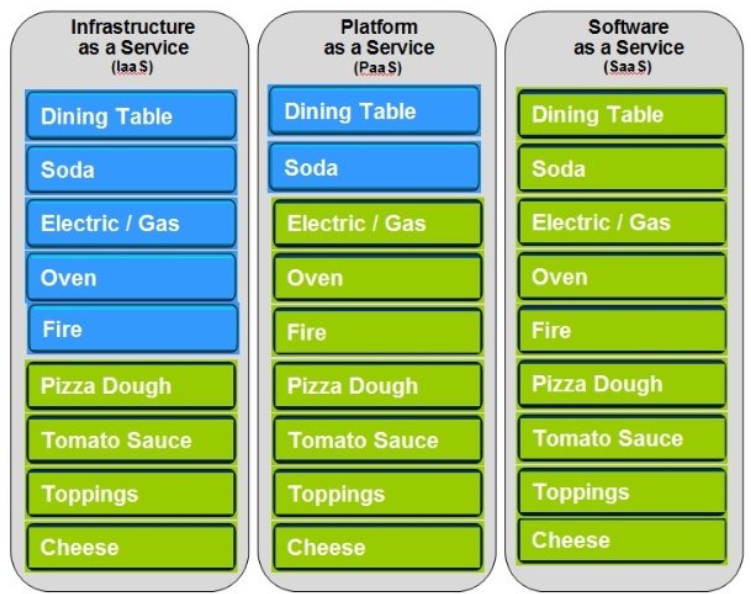
\includegraphics[width=0.80\linewidth,height=0.45\textheight,keepaspectratio]{images/05-cloud_fig5-3_pizza-as-a-service.png}
\caption{Pizza as a Service (in blu ciò che gestisce il cliente, in verde ciò che
gestisce il fornitore).}
\end{figure}

\subsection{SaaS}\label{saas}

Prima del SaaS i prodotti software si installavano sui computer dei
clienti. I clienti dovevano configurarli e gestirne gli aggiornamenti, e
le aziende dovevano mantenere diverse versioni del prodotto. Con il SaaS
il prodotto è fornito come servizio: il cliente non installa nulla, paga
un \textbf{abbonamento} e usa il prodotto da remoto.

Vantaggi del SaaS (per il fornitore):

\begin{itemize}
\tightlist
\item
  \textbf{Flusso di cassa}: entrate regolari, perché i clienti pagano
  abbonamenti periodici o a consumo.
\item
  \textbf{Gestione degli aggiornamenti}: è il fornitore a controllare
  gli aggiornamenti, e tutti i clienti li ricevono insieme. Non si
  devono mantenere più versioni, quindi si risparmia.
\item
  \textbf{Continuous deployment}: si possono rilasciare nuove versioni
  appena le modifiche sono pronte e testate.
\item
  \textbf{Flessibilità nei pagamenti}: diverse opzioni di pagamento
  attirano più clienti (es. piccole aziende o privati evitano grandi
  costi iniziali).
\item
  \textbf{Prova prima di comprare} (\emph{try before you buy}): si può
  offrire il prodotto gratis o a basso costo all'inizio per raccogliere
  feedback (es. gratis per qualche settimana).
\item
  \textbf{Raccolta dati}: è facile raccogliere dati su come viene usato
  il prodotto e su come interagiscono i clienti.
\end{itemize}

Svantaggi del SaaS:

\begin{itemize}
\tightlist
\item
  \textbf{Rispetto delle leggi sulla privacy}: ogni Paese ha leggi
  diverse, spesso severe, su dove e come conservare i dati personali.
\item
  \textbf{Sicurezza}: i clienti possono non voler cedere il controllo
  dei propri dati a un fornitore esterno, che però deve gestirli. E se
  il fornitore subisce un furto di dati (\emph{data breach}), avviserà i
  clienti?
\item
  \textbf{Limiti della rete}: possono rallentare le risposte quando si
  trasferiscono molti dati.
\item
  \textbf{Scambio di dati}: se il cloud non offre API adatte, scambiare
  dati è difficile. Dipende dal contratto: a seconda dell'offerta si può
  accedere a insiemi di dati diversi.
\item
  \textbf{Perdita di controllo sugli aggiornamenti}: il fornitore può
  cambiare troppo e troppo spesso (es. nuove funzioni ogni giorno che
  cambiano l'interfaccia).
\item
  \textbf{Service lock-in}: è difficile spostarsi da un fornitore SaaS a
  un altro.
\end{itemize}

Scelto il SaaS, bisogna affrontare alcune questioni di design:

\begin{itemize}
\tightlist
\item
  \textbf{Elaborazione locale o remota}: alcune feature si possono
  eseguire in locale, riducendo il traffico di rete e velocizzando le
  risposte, ma aumentando il consumo di batteria sui dispositivi mobili.
\item
  \textbf{Autenticazione}: di solito ci sono tre possibilità: un sistema
  di autenticazione proprio del prodotto; l'\textbf{autenticazione
  federata}, basata su un rapporto di fiducia tra un \emph{Service
  Provider} (SP, es. chi vende l'applicazione) e un \emph{Identity
  Provider} (IdP) esterno; le credenziali personali di servizi esterni
  (es. Google, LinkedIn).
\item
  \textbf{Fuga di informazioni} (\emph{information leakage}): se il
  servizio è offerto a più organizzazioni, c'è il rischio che un membro
  di un'organizzazione acceda a dati di un'altra.
\item
  \textbf{Database multi-tenant o multi-instance}: i sistemi
  \textbf{multi-tenant} usano un solo archivio (con tecniche avanzate
  per partizionare i dati e controllare le partizioni), quelli
  \textbf{multi-instance} hanno copie separate del sistema e del
  database per ogni cliente.
\end{itemize}

\subsection{Sistemi multi-tenant e
multi-instance}\label{sistemi-multi-tenant-e-multi-instance}

\subsubsection{Sistemi multi-tenant}\label{sistemi-multi-tenant}

\begin{boxdefinition}{Sistema multi-tenant}

Un sistema \textbf{multi-tenant} usa \textbf{un unico schema di
database} condiviso da tutti gli utenti. Ogni riga è etichettata con un
\textbf{identificatore del tenant} (il cliente): così si ottiene un
\textbf{isolamento logico}, cioè ogni utente vede solo i dati del
proprio tenant.

\end{boxdefinition}

\begin{figure}[H]
\centering
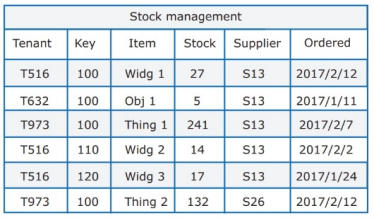
\includegraphics[width=0.60\linewidth,height=0.45\textheight,keepaspectratio]{images/05-cloud_fig5-4_schema-multi-tenant.png}
\caption{Esempio di schema di database multi-tenant.}
\end{figure}

Vantaggi:

\begin{itemize}
\tightlist
\item
  \textbf{Uso delle risorse}: il fornitore controlla tutte le risorse
  usate dal software e può ottimizzarle.
\item
  \textbf{Sicurezza}: siccome i dati di tutti i clienti stanno nello
  stesso database, il database deve essere progettato fin dall'inizio
  per la sicurezza, quindi probabilmente avrà meno vulnerabilità di un
  database standard. Inoltre c'è una sola copia del software da
  correggere se si scopre una vulnerabilità.
\item
  \textbf{Gestione degli aggiornamenti}: aggiornare un'unica istanza è
  più facile che aggiornarne tante, e tutti i clienti usano sempre
  l'ultima versione.
\end{itemize}

Svantaggi:

\begin{itemize}
\tightlist
\item
  \textbf{Poca flessibilità}: tutti i clienti devono usare lo stesso
  schema, con poche possibilità di adattarlo.
\item
  \textbf{Sicurezza}: con i dati di tutti nello stesso database, c'è il
  rischio teorico che i dati passino da un cliente all'altro. Peggio
  ancora, un attacco al database colpisce \textbf{tutti} i clienti.
\item
  \textbf{Complessità}: dover gestire tanti utenti rende questi sistemi
  più complessi dei multi-instance, e quindi più esposti a bug.
\end{itemize}

Le aziende medie e grandi raramente vogliono software multi-tenant
generico: preferiscono una versione adattata alle loro esigenze. Due
soluzioni possibili:

\begin{enumerate}
\def\labelenumi{\arabic{enumi}.}
\tightlist
\item
  \textbf{Aggiungere campi extra} a ogni tabella, che il cliente usa
  come vuole. Però è difficile prevedere quante colonne servono (troppo
  poche non bastano, troppe sprecano spazio) e clienti diversi vorranno
  tipi di colonne diversi.
\item
  \textbf{Aggiungere a ogni tabella un campo che punta a una ``tabella
  di estensione''}, che il cliente crea secondo le sue esigenze. Questo
  però aggiunge complessità a un sistema già complesso.
\end{enumerate}

La \textbf{sicurezza} è la preoccupazione principale dei clienti
aziendali. Poiché tutto sta nello stesso database, un bug o un attacco
potrebbe esporre i dati di alcuni o di tutti i clienti. Per ridurre il
rischio si usano:

\begin{itemize}
\tightlist
\item
  il \textbf{controllo degli accessi multilivello}: l'accesso ai dati è
  controllato sia a livello di organizzazione sia a livello del singolo
  utente;
\item
  la \textbf{cifratura dei dati}: così, se il sistema si guasta, i dati
  di un'azienda non sono leggibili da persone di altre aziende. Di
  solito si cifrano solo i dati sensibili.
\end{itemize}

\subsubsection{Sistemi multi-instance}\label{sistemi-multi-instance}

\begin{boxdefinition}{Sistema multi-instance}

In un sistema \textbf{multi-instance} ogni cliente ha il \textbf{proprio
sistema}, adattato alle sue esigenze, con il proprio database e i propri
controlli di sicurezza.

\end{boxdefinition}

È concettualmente più semplice di un sistema multi-tenant ed elimina
problemi come la fuga di dati tra organizzazioni. Si può realizzare in
due modi:

\begin{itemize}
\tightlist
\item
  \textbf{Basato su VM}: l'istanza del software e il database di ogni
  cliente girano in una propria macchina virtuale. Tutti gli utenti
  dello stesso cliente accedono al database condiviso di quel sistema.
\item
  \textbf{Basato su container}: ogni utente ha una versione isolata del
  software e del database, in un insieme di container. È la soluzione
  migliore per prodotti in cui gli utenti lavorano per lo più da soli,
  condividendo pochi dati (es. utenti privati).
\end{itemize}

Le due cose si possono anche combinare: un'azienda può avere il proprio
sistema su VM e, sopra, eseguire container per i singoli utenti.

Vantaggi:

\begin{itemize}
\tightlist
\item
  \textbf{Flessibilità}: ogni istanza si può adattare alle esigenze del
  cliente.
\item
  \textbf{Sicurezza}: ogni cliente ha il suo database, quindi niente
  fughe di dati tra clienti.
\item
  \textbf{Scalabilità}: ogni istanza si scala secondo le esigenze del
  suo cliente (qualcuno avrà bisogno di server più potenti di altri).
\item
  \textbf{Resilienza}: un guasto software probabilmente colpisce un solo
  cliente, gli altri continuano a lavorare.
\end{itemize}

Svantaggi:

\begin{itemize}
\tightlist
\item
  \textbf{Costo}: affittare tante VM nel cloud e gestire tanti sistemi
  costa di più. Le VM si avviano lentamente, quindi spesso vanno tenute
  accese sempre, anche quando il servizio è poco usato.
\item
  \textbf{Gestione degli aggiornamenti}: aggiornare tante istanze è
  complicato, soprattutto se sono state personalizzate per clienti
  diversi.
\end{itemize}

\section{Architettura del software nel
cloud}\label{architettura-del-software-nel-cloud}

Nelle prime fasi del design di un'architettura cloud bisogna rispondere
ad alcune domande:

\begin{itemize}
\tightlist
\item
  Database \textbf{multi-tenant o multi-instance}? (organizzazione del
  database)
\item
  Quali sono i requisiti di \textbf{scalabilità e resilienza}?
\item
  Struttura \textbf{monolitica o a servizi}? (struttura del software)
\end{itemize}

Le risposte guidano la scelta della piattaforma cloud su cui installare
e distribuire il prodotto.

\subsection{Organizzazione del
database}\label{organizzazione-del-database}

Ci sono tre modi per fornire il database dei clienti in un sistema
cloud:

\begin{enumerate}
\def\labelenumi{\arabic{enumi}.}
\tightlist
\item
  \textbf{Multi-tenant}, condiviso da tutti i clienti e ospitato nel
  cloud su server grandi e potenti.
\item
  \textbf{Multi-instance}, con il database di ogni cliente in una
  propria macchina virtuale.
\item
  \textbf{Multi-instance}, con ogni database in un proprio container. Il
  database di un cliente può anche essere distribuito su più container.
\end{enumerate}

Fattori per scegliere:

\begin{itemize}
\tightlist
\item
  \textbf{Clienti target}: i clienti hanno bisogno di schemi di database
  diversi e di personalizzazioni? Se sì → \textbf{multi-instance}.
\item
  \textbf{Requisiti sulle transazioni}: è fondamentale supportare
  transazioni \textbf{ACID}, cioè avere dati sempre consistenti? Se sì →
  \textbf{multi-tenant} o \textbf{multi-instance su VM}.
\item
  \textbf{Dimensione e connessioni del database}: quanto è grande il
  database tipico? Quante relazioni ci sono tra i dati? Per database
  molto grandi di solito conviene il \textbf{multi-tenant}, perché si
  possono concentrare gli sforzi sull'ottimizzazione delle prestazioni.
\item
  \textbf{Interoperabilità}: i clienti vorranno trasferire dati da
  database esistenti? Quanto sono diversi i loro schemi da un possibile
  schema multi-tenant? Che supporto si aspettano per il trasferimento?
  Se i clienti hanno schemi molto diversi → \textbf{multi-instance}.
\item
  \textbf{Struttura del sistema}: si usa un'architettura a servizi? Il
  database del cliente si può dividere in tanti database, uno per
  servizio? Se sì → \textbf{multi-instance in container}.
\end{itemize}

\subsection{Scalabilità e resilienza}\label{scalabilituxe0-e-resilienza}

\subsubsection{Scalabilità}\label{scalabilituxe0}

La \textbf{scalabilità} (la capacità di adattarsi automaticamente ai
cambiamenti di carico) si ottiene in due modi quando il carico cresce:

\begin{itemize}
\tightlist
\item
  \textbf{scaling out} (scalare in orizzontale): aggiungere nuovi server
  virtuali;
\item
  \textbf{scaling up} (scalare in verticale): aumentare la potenza di un
  server esistente.
\end{itemize}

Nel cloud si fa tipicamente \textbf{scaling out}: il prodotto deve
essere organizzato in modo che i singoli componenti si possano replicare
ed eseguire in parallelo, mentre dei meccanismi di \textbf{load
balancing} distribuiscono le richieste tra le istanze (ad esempio con un
PaaS).

\subsubsection{Resilienza}\label{resilienza}

La \textbf{resilienza} (la capacità di continuare a fornire i servizi
critici in caso di guasti o attacchi) si ottiene con la tecnica
dell'\textbf{hot standby}: si tengono \textbf{repliche} del software e
dei dati in luoghi diversi (Fig. 5.5). Gli aggiornamenti del database
vengono copiati sull'altro database (\emph{mirroring}) e un
\textbf{system monitor} controlla di continuo lo stato del sistema.

Un'alternativa più economica è il \textbf{cool standby}: in caso di
guasto i dati si ripristinano da un backup, quindi il sistema resta non
disponibile finché il ripristino non è finito.

\begin{figure}[H]
\centering
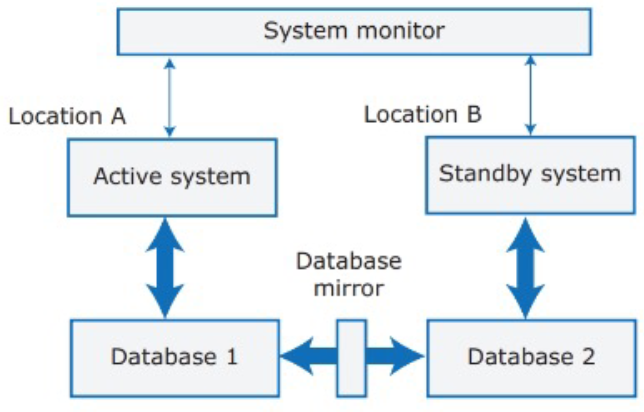
\includegraphics[width=0.60\linewidth,height=0.45\textheight,keepaspectratio]{images/05-cloud_fig5-5_hot-standby.png}
\caption{Schema della tecnica hot standby.}
\end{figure}

\subsection{Struttura del software}\label{struttura-del-software}

La scelta principale è tra un sistema \textbf{monolitico} e
\textbf{servizi piccoli e senza stato} (\emph{fine-grained, stateless}).
I servizi indipendenti si possono replicare, distribuire e spostare,
quindi sono particolarmente adatti al software cloud con servizi in
container. Il monolite si usa spesso per costruire i \textbf{prototipi},
anche quando alla fine un sistema a servizi sarebbe più adatto.

Per scegliere la piattaforma cloud si considerano due gruppi di aspetti:

\begin{enumerate}
\def\labelenumi{\arabic{enumi}.}
\tightlist
\item
  \textbf{Aspetti tecnici}: carico previsto e quanto è prevedibile,
  resilienza, servizi cloud offerti dal provider, privacy e protezione
  dei dati (alcuni Paesi UE hanno regole severe su come e dove si
  salvano i dati, quindi il provider deve garantire dove vengono
  conservati).
\item
  \textbf{Aspetti di business}: esperienza degli sviluppatori (linguaggi
  e tecnologie dipendono da cosa sa il team), \textbf{Service Level
  Agreement} (SLA, le garanzie offerte dal provider), portabilità e
  migrazione (avere un ``piano d'uscita'' contro il vendor lock-in),
  clienti target (che magari hanno sistemi vecchi che devono interagire
  con i nuovi) e costi (inclusi quelli per sviluppatori e tecnologie).
\end{enumerate}

\section{Orchestrazione dei
container}\label{orchestrazione-dei-container}

Come visto, i container sono un modo leggero per isolare l'ambiente di
un'applicazione. Le immagini dei container si possono eseguire in modo
affidabile su qualsiasi macchina, garantendo portabilità dallo sviluppo
al deploy (noi abbiamo usato Docker).

Il deploy automatico che offre Docker, però, ha poche capacità di
ottimizzare l'uso della memoria e può non sfruttare bene le risorse. E
restano varie domande aperte:

\begin{itemize}
\tightlist
\item
  Cosa succede se un container muore?
\item
  Cosa succede se si guasta la macchina su cui gira il container?
\item
  Come comunicano più container tra loro, anche su nodi diversi?
\item
  Come si gestisce la rete tra container?
\item
  Se la produzione ha più macchine, come si decide su quale far girare
  un container?
\end{itemize}

La soluzione è l'\textbf{orchestrazione dei container}: l'architetto
definisce quali container devono girare e poi lascia alla piattaforma di
orchestrazione il compito di realizzare quella configurazione.

\subsection{Kubernetes}\label{kubernetes}

Una delle piattaforme di orchestrazione più usate è \textbf{Kubernetes}
(abbreviato \textbf{K8s}). Gestisce l'intero ciclo di vita dei
container, creando e spegnendo risorse quando serve: se un container si
spegne all'improvviso, K8s ne lancia un altro al suo posto. Offre anche
un meccanismo per far comunicare le applicazioni tra loro anche mentre i
container sottostanti vengono creati e distrutti. Dato un insieme di
carichi di lavoro (container) e un insieme di macchine in un
\textbf{cluster}, l'orchestratore esamina ogni container e sceglie la
macchina migliore su cui eseguirlo.

Kubernetes riceve tramite la sua API lo \textbf{stato desiderato}
(\emph{Desired State Management}), descritto in un \textbf{manifest}
YAML. Il manifest dice quali sono i \textbf{Pod} (gruppi di container) e
quante \textbf{repliche} di ciascuno servono. Kubernetes mette sullo
stesso nodo tutti i container di uno stesso Pod e crea tante repliche
quante ne sono richieste; un nodo può ospitare più Pod. Se un nodo
(\emph{worker}, cioè una macchina che ospita container) si guasta,
Kubernetes se ne accorge e avvia una nuova replica altrove (Fig. 5.6). I
servizi del cluster Kubernetes gestiscono anche la comunicazione tra i
nodi, sia quelli esistenti sia quelli nuovi.

\begin{figure}[H]
\centering
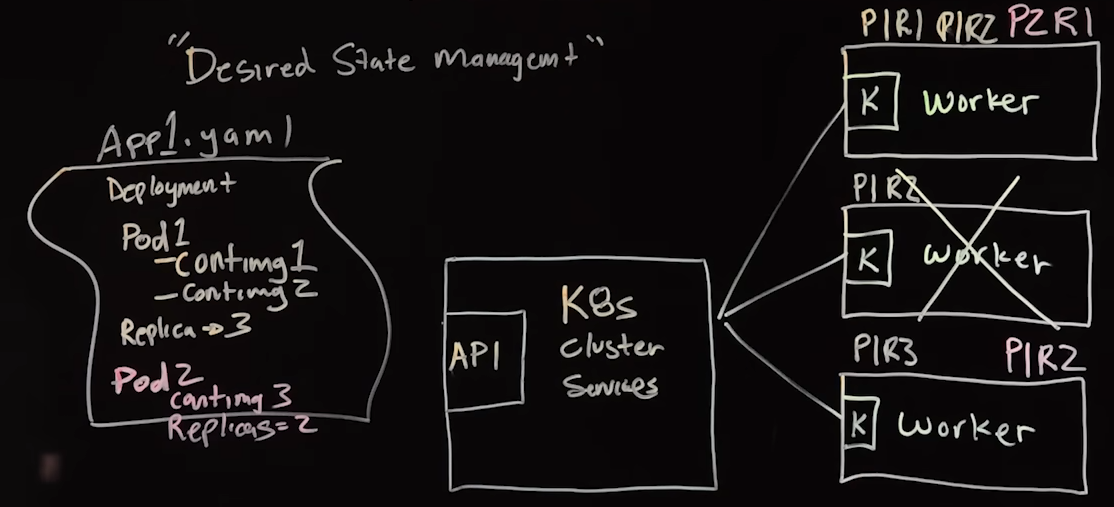
\includegraphics[width=0.80\linewidth,height=0.45\textheight,keepaspectratio]{images/05-cloud_fig5-6_idea-kubernetes.png}
\caption{L'idea di gestione di Kubernetes.}
\end{figure}

\begin{boxexample}{Un manifest minimo (Deployment)}

Questo manifest chiede a K8s di tenere sempre attive 3 repliche di un
Pod con un container \texttt{web}:

\begin{Verbatim}
apiVersion: apps/v1
kind: Deployment
metadata:
  name: web
spec:
  replicas: 3
  selector:
    matchLabels: { app: web }
  template:
    metadata:
      labels: { app: web }
    spec:
      containers:
        - name: web
          image: nginx:1.27
\end{Verbatim}

Se un Pod muore, K8s nota che le repliche sono 2 invece di 3 e ne crea
una nuova.

\end{boxexample}

\subsection{Principi di design di
Kubernetes}\label{principi-di-design-di-kubernetes}

\begin{itemize}
\tightlist
\item
  \textbf{Dichiaratività}: con l'approccio dichiarativo si descrive solo
  lo \textbf{stato desiderato} del sistema (nel manifest). K8s si
  accorge quando lo stato reale non corrisponde a quello desiderato e
  interviene per correggerlo: il sistema diventa \textbf{self-healing}
  (si ripara da solo). Lo stato desiderato è definito da un insieme di
  \textbf{oggetti}: ogni oggetto ha una \textbf{specifica} (\emph{spec},
  lo stato desiderato) e uno \textbf{stato} (\emph{status}, lo stato
  attuale). K8s controlla di continuo che lo stato di ogni oggetto sia
  uguale alla specifica: se un oggetto non risponde ne avvia una nuova
  versione; se il suo stato si è allontanato dalla specifica, esegue i
  comandi necessari per riportarlo allo stato desiderato.
\item
  \textbf{Distribuzione}: Kubernetes offre un'\textbf{unica interfaccia}
  per interagire con un intero cluster di macchine, così gli
  sviluppatori non devono comunicare con ogni macchina singolarmente.
\end{itemize}

\begin{figure}[H]
\centering
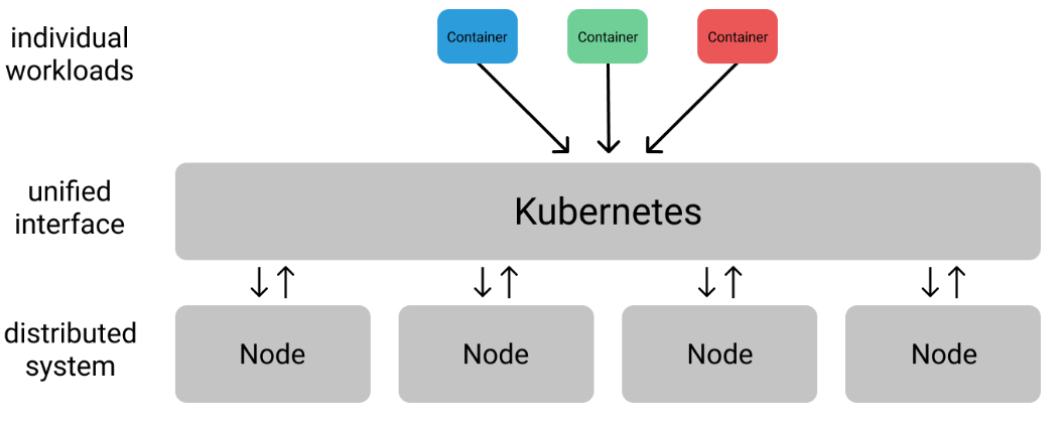
\includegraphics[width=0.75\linewidth,height=0.45\textheight,keepaspectratio]{images/05-cloud_fig5-7_distribuzione-k8s.png}
\caption{Schema della distribuzione in Kubernetes.}
\end{figure}

\begin{itemize}
\tightlist
\item
  \textbf{Disaccoppiamento}: ogni container dovrebbe occuparsi di
  \textbf{una sola cosa}, come nelle architetture a microservizi. K8s
  supporta in modo naturale servizi disaccoppiati, che si possono
  scalare e aggiornare in modo indipendente.
\item
  \textbf{Infrastruttura immutabile}: invece di entrare in un container
  per aggiornare una libreria, si costruisce una \textbf{nuova
  immagine}, si installa la nuova versione e si spegne quella vecchia.
  Il motivo è che i container sono pensati per essere \textbf{effimeri},
  pronti a essere sostituiti in qualsiasi momento. Un'infrastruttura
  immutabile rende anche facile tornare a uno stato precedente (es. dopo
  un errore): basta cambiare la configurazione per usare un'immagine più
  vecchia.
\end{itemize}

\subsection{Oggetti di Kubernetes}\label{oggetti-di-kubernetes}

Kubernetes definisce molti oggetti che si possono descrivere nei
manifest (in JSON o YAML). I principali sono:

\begin{itemize}
\tightlist
\item
  \textbf{Pod}: la \textbf{più piccola unità di deploy} di Kubernetes. È
  formato da uno o più container strettamente collegati, con una rete e
  dei volumi (file system) condivisi. Un Pod non si distribuisce su più
  macchine. Ogni Pod ha un \textbf{indirizzo IP} unico per comunicare
  con lui.
\end{itemize}

\begin{figure}[H]
\centering
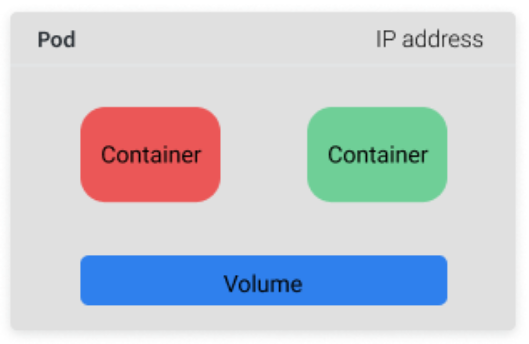
\includegraphics[width=0.60\linewidth,height=0.45\textheight,keepaspectratio]{images/05-cloud_fig5-8_pod.png}
\caption{Schema di un Pod.}
\end{figure}

\begin{itemize}
\tightlist
\item
  \textbf{Deployment}: un insieme di Pod definito da un
  \textbf{template} e da un \textbf{numero di repliche} \emph{n} (quante
  copie del template far girare). Il cluster cerca sempre di avere
  \emph{n} Pod disponibili.
\end{itemize}

\begin{figure}[H]
\centering
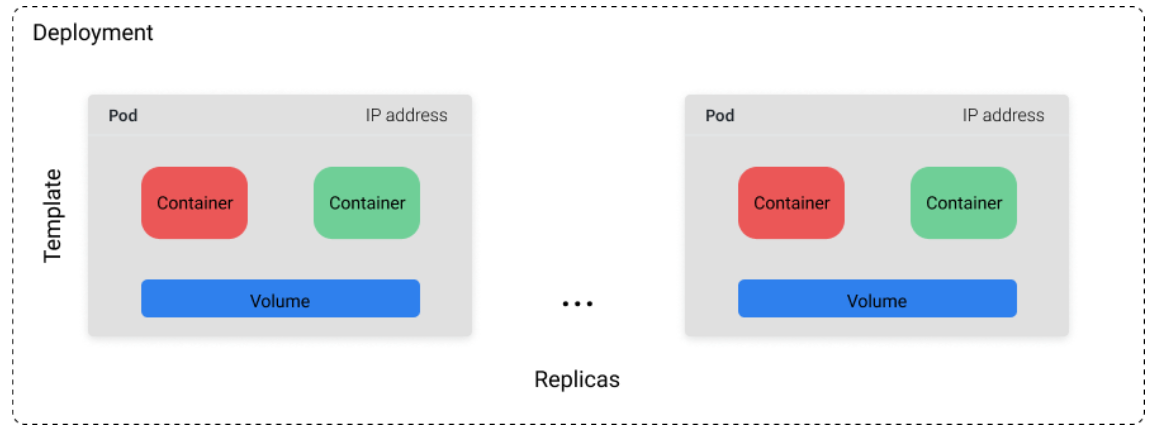
\includegraphics[width=1.00\linewidth,height=0.45\textheight,keepaspectratio]{images/05-cloud_fig5-9_deployment.png}
\caption{Schema di un Deployment.}
\end{figure}

\begin{itemize}
\tightlist
\item
  \textbf{Service}: offre un \textbf{punto di accesso stabile} per
  mandare il traffico ai Pod giusti, anche quando i Pod cambiano per
  aggiornamenti, scaling o guasti. Il Service sa a quali Pod inviare il
  traffico grazie alle \textbf{label} (coppie chiave-valore) definite
  nei metadati dei Pod.
\end{itemize}

\begin{figure}[H]
\centering
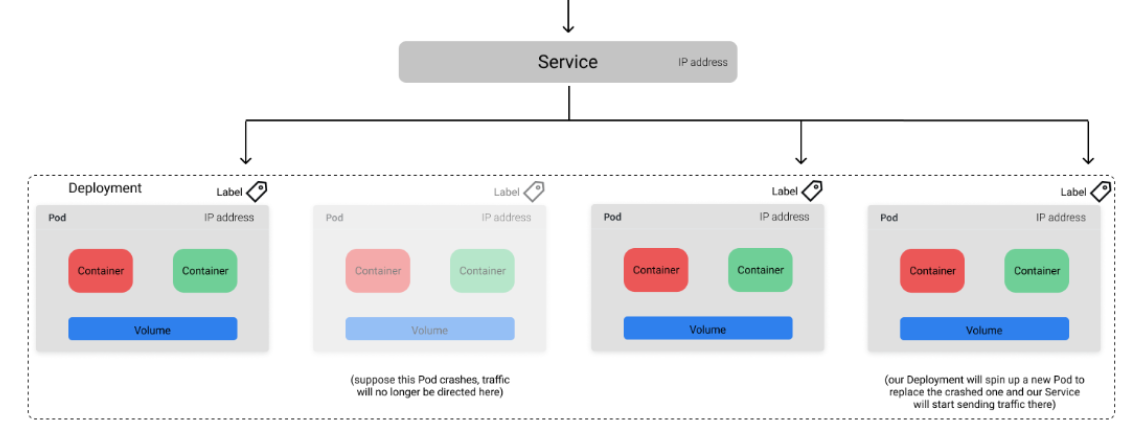
\includegraphics[width=1.00\linewidth,height=0.45\textheight,keepaspectratio]{images/05-cloud_fig5-10_service.png}
\caption{Schema di un Service.}
\end{figure}

\begin{itemize}
\tightlist
\item
  \textbf{Ingress}: i Service sono raggiungibili solo dall'interno del
  cluster. Per esporre l'applicazione al \textbf{traffico esterno} si
  definisce un oggetto Ingress, che sceglie quali Service rendere
  pubblici e li espone dietro un punto di accesso stabile (un URL
  esterno).
\end{itemize}

\begin{figure}[H]
\centering
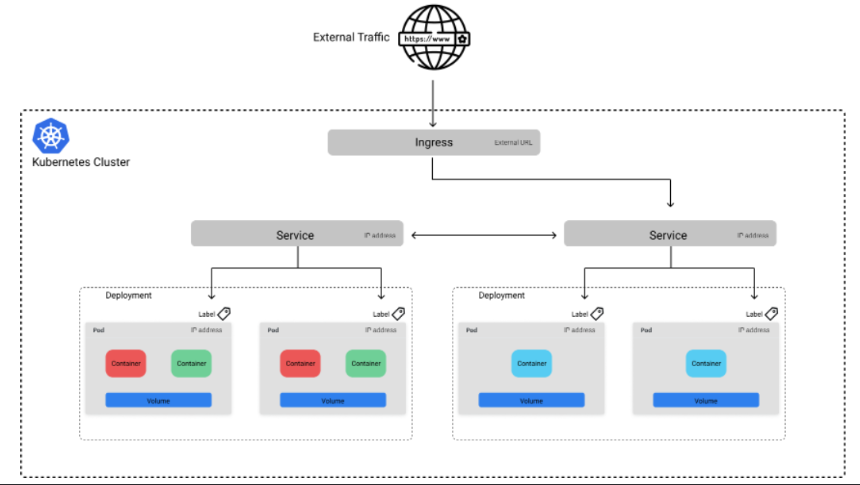
\includegraphics[width=1.00\linewidth,height=0.45\textheight,keepaspectratio]{images/05-cloud_fig5-11_ingress.png}
\caption{Schema di un Ingress.}
\end{figure}

\subsection{Il control plane di
Kubernetes}\label{il-control-plane-di-kubernetes}

Vediamo ad alto livello come funziona Kubernetes ``sotto il cofano''. Un
cluster (insieme di macchine) ha due tipi di macchine:

\begin{itemize}
\tightlist
\item
  il \textbf{master node} (spesso uno solo), che contiene la maggior
  parte dei componenti del \textbf{control plane};
\item
  i \textbf{worker node}, che eseguono i carichi di lavoro delle
  applicazioni.
\end{itemize}

\subsubsection{Master node}\label{master-node}

Gli utenti inviano le specifiche nuove o aggiornate degli oggetti (i
manifest) all'\textbf{API server} del master node. L'API server valida
le richieste (controllando l'input) e fa da \textbf{interfaccia unica}
per qualsiasi domanda sullo stato attuale del cluster. Lo stato del
cluster (configurazione, specifiche e stati degli oggetti, nodi del
cluster, assegnazione degli oggetti ai nodi, \ldots) è salvato in un
archivio chiave-valore distribuito chiamato \textbf{etcd}.

Il master node (Fig. 5.12) è formato da:

\begin{itemize}
\tightlist
\item
  l'\textbf{API server};
\item
  \textbf{etcd}, che contiene tutto lo stato del cluster;
\item
  il \textbf{controller-manager};
\item
  lo \textbf{scheduler}.
\end{itemize}

L'API server fa da intermediario per rispettare il principio di
\textbf{disaccoppiamento}: ogni componente ha un solo compito, e questo
rende anche più facile ripartire dopo un guasto.

Il \textbf{controller-manager} controlla lo stato del cluster tramite
l'API server. Se lo stato reale è diverso da quello desiderato, chiede
modifiche all'API server per portare il cluster verso lo stato
desiderato.

\begin{figure}[H]
\centering
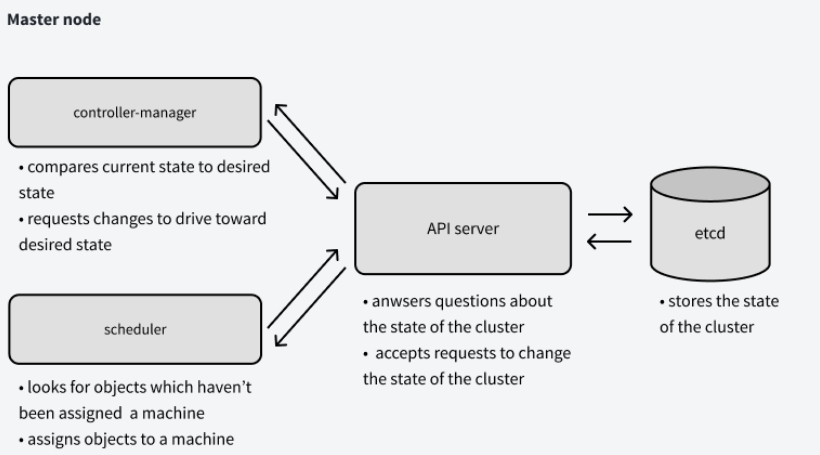
\includegraphics[width=1.00\linewidth,height=0.45\textheight,keepaspectratio]{images/05-cloud_fig5-12_master-node.png}
\caption{Struttura del master node di Kubernetes.}
\end{figure}

Lo \textbf{scheduler} decide dove eseguire gli oggetti (Fig. 5.13):

\begin{enumerate}
\def\labelenumi{\arabic{enumi}.}
\tightlist
\item
  chiede all'API server quali oggetti non sono ancora assegnati a una
  macchina;
\item
  l'API server gli restituisce gli oggetti non assegnati (letti da
  etcd);
\item
  lo scheduler decide a quali macchine assegnarli e lo comunica all'API
  server;
\item
  l'API server registra l'assegnazione in etcd.
\end{enumerate}

\begin{figure}[H]
\centering
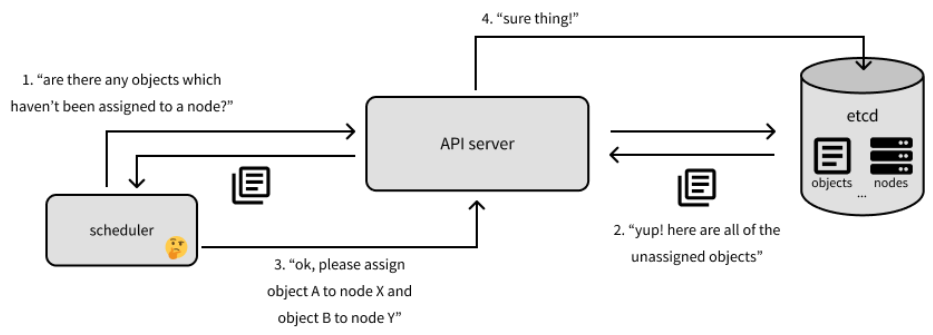
\includegraphics[width=1.00\linewidth,height=0.45\textheight,keepaspectratio]{images/05-cloud_fig5-13_scheduler.png}
\caption{Il ciclo di vita dello scheduler.}
\end{figure}

\subsubsection{Worker node}\label{worker-node}

Ogni worker node contiene un \textbf{kubelet}, l'\,``agente'' del nodo:
comunica con l'API server per sapere quali container sono stati
assegnati al nodo ed è responsabile di avviare i Pod che li eseguono.
Quando un nodo entra nel cluster, il kubelet annuncia la sua esistenza
all'API server, così lo scheduler può assegnargli dei Pod. Ogni worker
contiene anche \textbf{kube-proxy}, che permette ai container di
comunicare tra loro attraverso i vari nodi del cluster. La Fig. 5.14
mostra la struttura completa.

\begin{figure}[H]
\centering
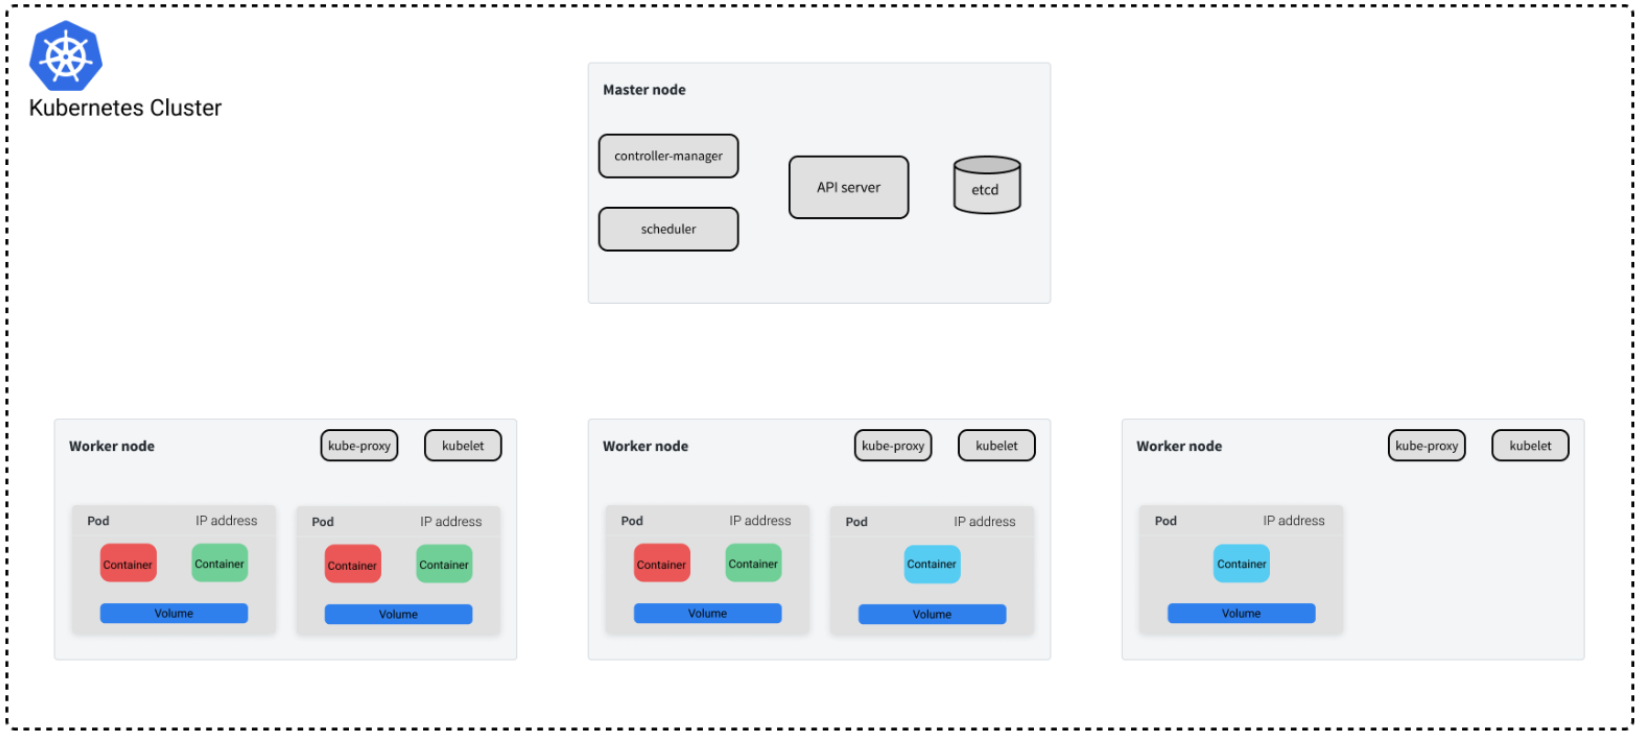
\includegraphics[width=1.00\linewidth,height=0.45\textheight,keepaspectratio]{images/05-cloud_fig5-14_struttura-k8s.png}
\caption{La struttura completa di Kubernetes.}
\end{figure}

\begin{boxwarning}{Quando Kubernetes non conviene}

\begin{itemize}
\tightlist
\item
  Se il carico di lavoro può girare su \textbf{una sola macchina}.
\item
  Se serve \textbf{poca potenza di calcolo}.
\item
  Se non serve \textbf{alta disponibilità} e si possono tollerare
  periodi di fermo.
\item
  Se non si prevede di \textbf{cambiare spesso} i servizi installati.
\item
  Se si ha un \textbf{monolite} e non si pensa di dividerlo in
  microservizi.
\end{itemize}

\end{boxwarning}

Esiste anche un modo per orchestrare container con Docker, chiamato
\textbf{Docker Swarm}, ma Kubernetes è un orchestratore molto più
potente. Le due tecnologie comunque collaborano, quindi non c'è lock-in
tra Docker e Kubernetes.
